% -------------------------------------------------------------------------
\begin{frame}{An Industry Case Study: Image Processing with SYCL}
  \begin{columns}
    \begin{column}{0.48\textwidth}
      The erosion morphologic operation:
        \begin{itemize}
          \item Lowest value from the neighbourhood
          \item Dark regions get bigger
          \item Bright regions shrink
        \end{itemize}
      \end{column}
      \begin{column}{0.48\textwidth}
        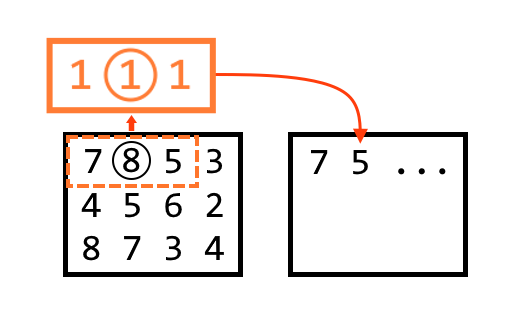
\includegraphics[width=\linewidth]{Images/erosion_graph.png}
      \end{column}
    \end{columns}
    Wooptix proposed to implement this algorithm.
\end{frame}
% -------------------------------------------------------------------------
\begin{frame}{An Industry Case Study: Image Processing with SYCL}
  \lstinputlisting[language=C++,style=cppstyle,title={Partial serial erosion code. \href{{https://github.com/AdrianoMoreira08/TFG-SYCL/blob/main/image-processing/morphology-gray/include/erode.h}}{\textit{See on Github}}}]{Code/serial-morph.cc}
\end{frame}
% -------------------------------------------------------------------------
\begin{frame}{An Industry Case Study: Image Processing with SYCL}
  \lstinputlisting[language=C++,style=cppstyle,title={Memory tiling code for SYCL erosion. \href{{https://github.com/AdrianoMoreira08/TFG-SYCL/blob/main/image-processing/morphology-gray/include/erode_sycl.h}}{\textit{See on Github}}}]{Code/sycl-morph-tile.cc}
\end{frame}
% -------------------------------------------------------------------------
\begin{frame}{An Industry Case Study: Image Processing with SYCL}
  \lstinputlisting[language=C++,style=cppstyle,title={Operation code for SYCL erosion. \href{{https://github.com/AdrianoMoreira08/TFG-SYCL/blob/main/image-processing/morphology-gray/include/erode_sycl.h}}{\textit{See on Github}}}]{Code/sycl-morph-op.cc}
\end{frame}
% -------------------------------------------------------------------------
\begin{frame}{An Industry Case Study: Image Processing with SYCL}
  \begin{figure}[H]
    \centering
    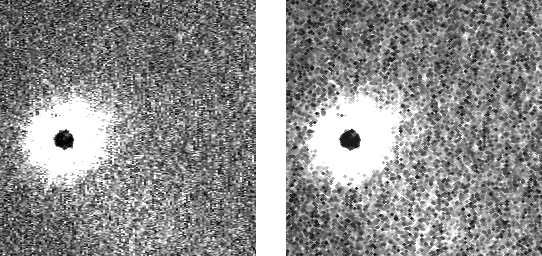
\includegraphics[width=0.7\linewidth]{Images/FOC-result.png}

    Sample from the Faint Object Camera from the Hubble Space Telescope.
    
    Original (left) and eroded (right).
  \end{figure}
  \begin{itemize}
    \item \textbf{Program time}: 1.10 sec. for serial and 1.30 sec. for SYCL
    \item \textbf{Algorithm time}: 0.04 sec. for serial and 0.17 sec. for SYCL
  \end{itemize}
\end{frame}
% -------------------------------------------------------------------------
\begin{frame}{An Industry Case Study: Image Processing with SYCL}
  \begin{figure}[H]
    \centering
    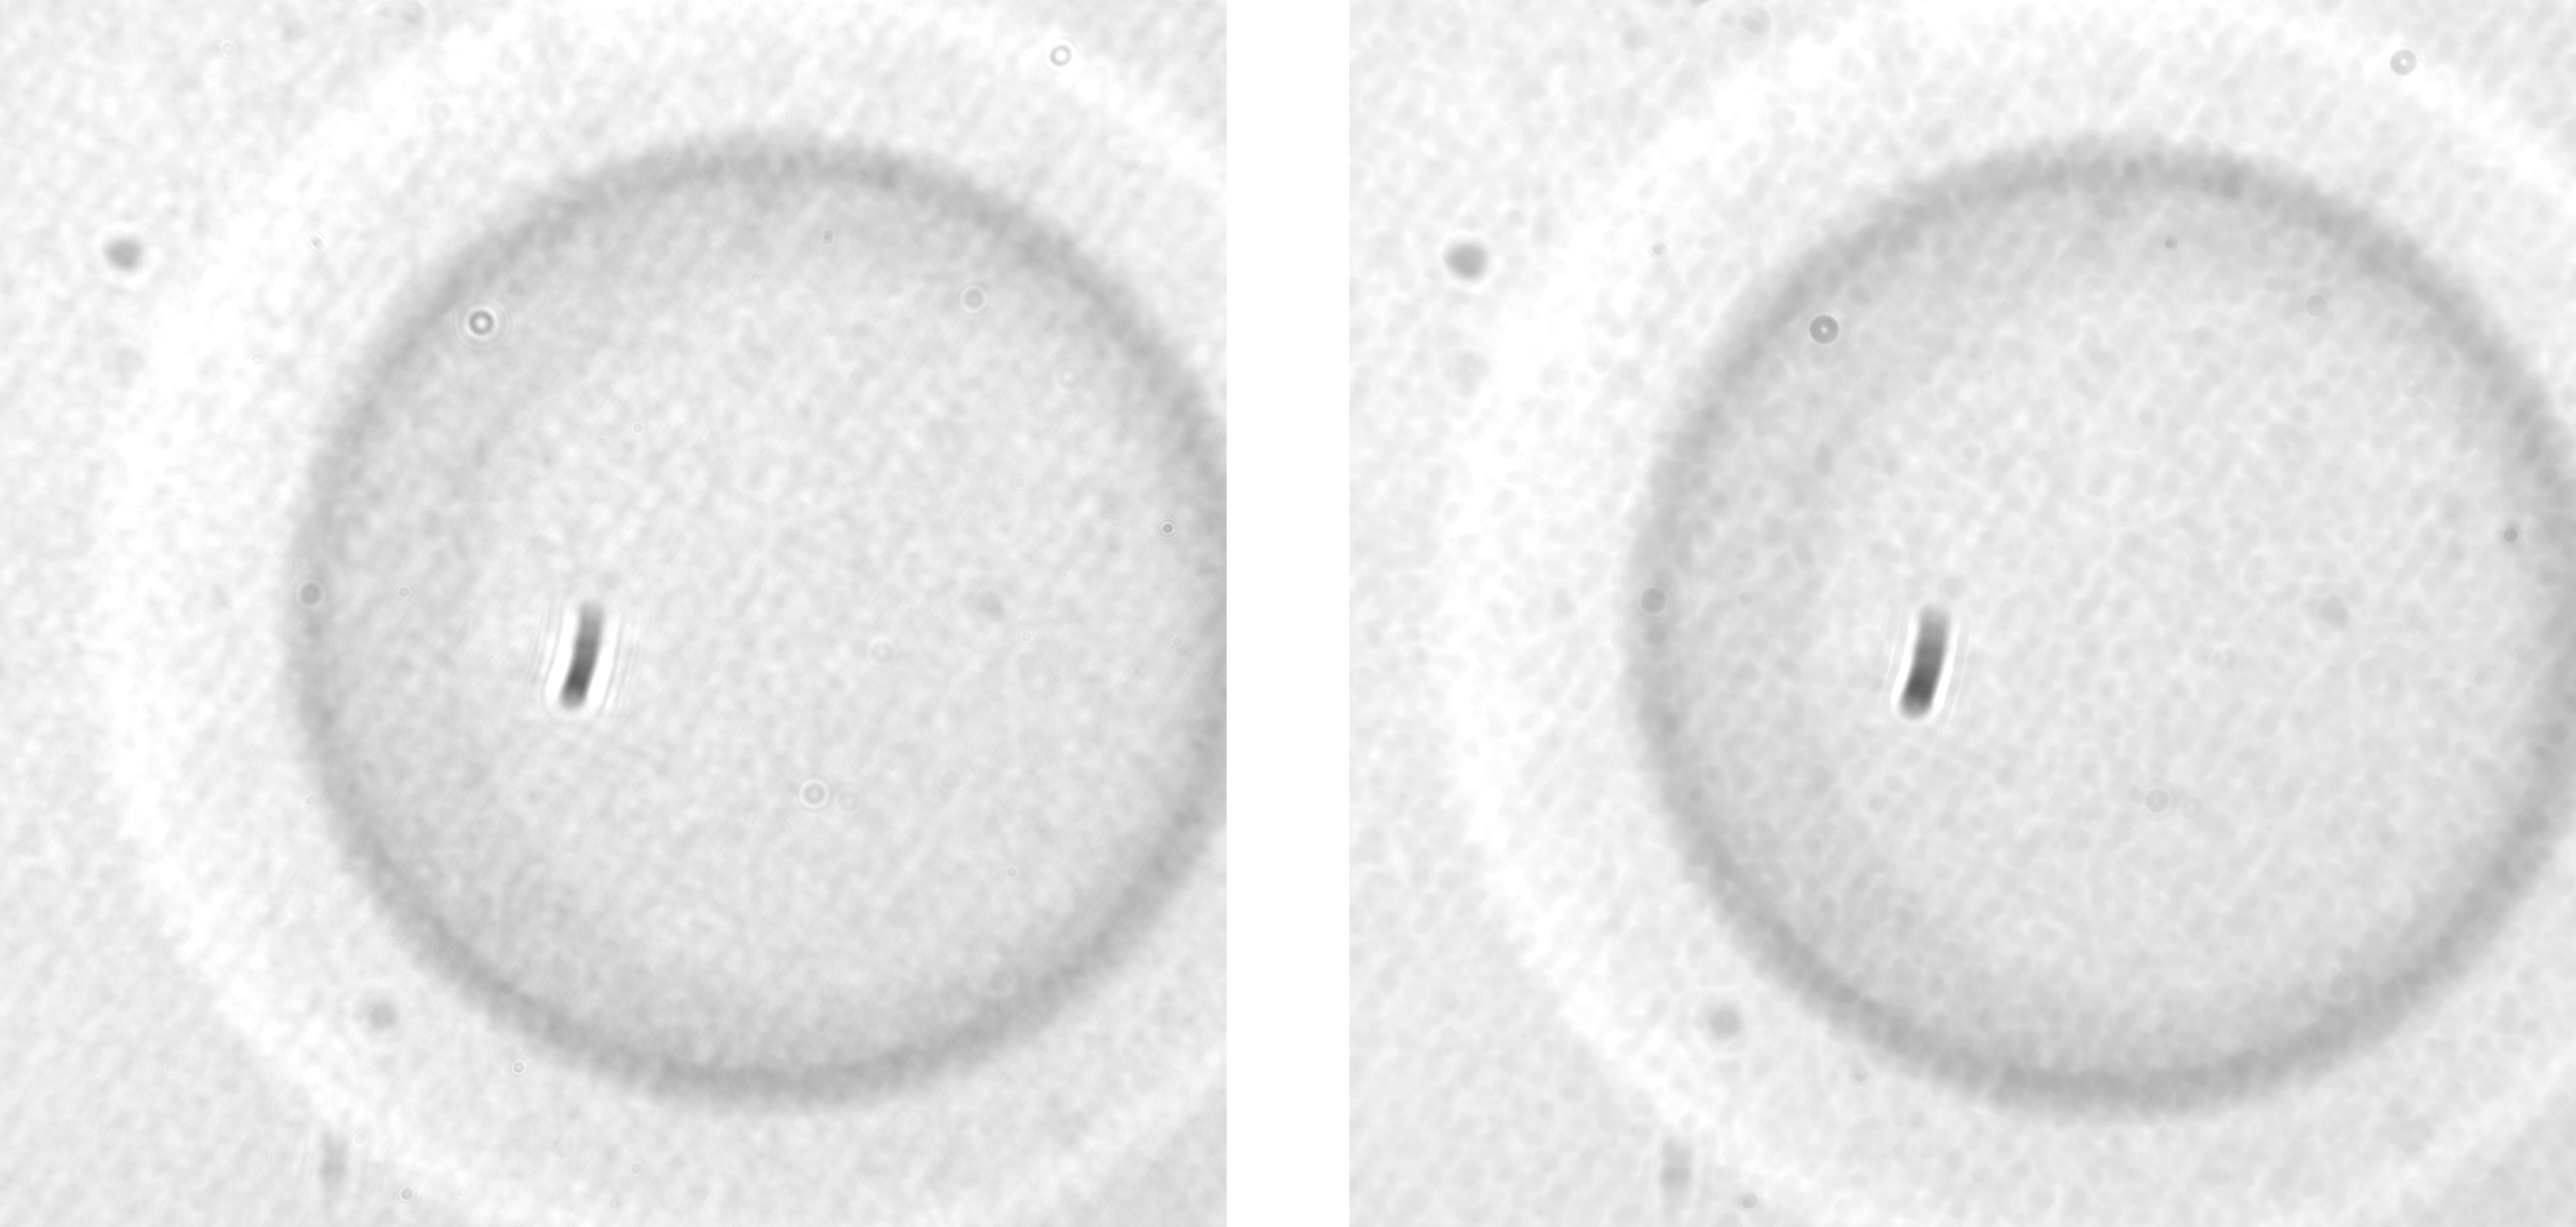
\includegraphics[width=0.7\linewidth]{Images/comparison-wooptix.png}

    Large sample image provided by Wooptix.
    
    Original (left) and eroded (right).
  \end{figure}
  \begin{itemize}
    \item \textbf{Program time}: 58.61 sec. for serial and 56.30 sec. for SYCL
    \item \textbf{Algorithm time}: 3.32 sec. for serial and 0.29 sec. for SYCL
  \end{itemize}
\end{frame}
% -------------------------------------------------------------------------